% !TEX root = ../thesis.tex
\chapter{基于相容条件概率分布重构的相似性学习}
\section{引言}
如前文所述,约束传播方法多数为针对单模态情况而设计的。近年来,有大量的工作对多模态融合进行了深入的研究\cite{lahat2015multimodal,poria2017ensemble,yu2017deep,poria2017review,liu2018weakly,kiela2018efficient}。在无监督或半监督的多模态任务中,学习的核心阻碍是训练数据不足而难以学习不同模态的权重。
模态权重表示了每种模态的重要性,因此,一些工作主张如果我们可以获得关于模态的先验知识,则可以为噪声较大的模态分配较小的权重\cite{kumar2011co,liu2013multi}。

在前文中我们所提出的MFL算法将模态级的融合学习推广到了多模态约束传播问题中。但是,通常情况下从模态的鲁棒性推导得出模态权重是更加合理。Sohn等人提出了一种深度学习方法以最小化两种模态之间的信息差异\cite{sohn2014improved},这可以视为通过鲁棒性学习模态融合的特殊情况。同时在鲁棒相似性矩阵学习方面也存在一些进展\cite{pavan2007dominant,premachandran2013consensus,zhu2014constructing}。这些方法
提供了不同的标准来衡量每个模态信息是否有噪声,而我们可以利用这些方法来生成模态的一些先验知识。

在本文中,我们首先提出了相容条件概率分布重构(Compatible Conditional Distributions Reconstruction,CCDR)这个基础问题,并给出了一个解决方案。基于CCDR,我们设计了一种新的多模态约束传播相似性学习方法,被命名为实例级多模态约束传播(Instance Level Multi-Modal Constraint Propagation,ILMCP)。
ILMCP会根据从每个模态上学习到的实例级的鲁棒性,为约束传播生成出统一的相似性图。所提出的方法将关注点集中在多模态约束传播中的转移概率推理上。
此外,区别于先前的工作,我们在本章所提出的方法建立在数据实例的邻域鲁棒性上,而不是每个模态整体的鲁棒性。为此,我们在算法中对成对的相容条件概率分布进行了重构,即给定特定数据实例条件下的模态概率以及给定某个模态条件下的特定数据实例的概率。随后,我们从上述分布中得出统一的转移概率,以生成一个相似性矩阵。除此之外,我们引入了一种代价敏感(cost-sensitive)的方法来平衡传播过程中的正约束和负约束数量问题。在数学符号表示上我们将延续上一章中的设定。

\section{相容条件概率分布重构}
在本节中,我们提出在特定假设下条件概率相容的必要和充分条件,并提出用于相容条件概率分布重构(Compatible Conditional Distributions Reconstruction,CCDR)的方法。

在许多实际情况下,条件分布比联合分布更加易于直观理解。研究人员更倾向于在提出的方法中采用一组假定存在的条件分布族,例如$P(X|Y)$和$P(Y|X)$\cite{arnold1989compatible}。但是,可能并不存在能够生成特定条件分布族的相关联的边缘概率分布和联合概率分布,这种情况被称为条件概率分布不相容。为了更准确的描述这种情况,我们在下文中给出了相容条件概率分布的定义。

\begin{definition}
    对于两个候选的条件概率分布族$ P(X|Y) $ 和 $ P(Y|X) $,如果存在一个与两者相关联的 $ (X,Y) $的联合概率分布,则称两个候选条件概率分布族为相容,否则称两个候选条件概率分布族不相容。
\end{definition}

条件概率分布相容性的充分必要条件由Arnold等人在文献\parencite{arnold1989compatible}中首次提出。由于文献\parencite{arnold1989compatible}中提出的条件针对于概率分布的一般情况,该条件对两个条件概率分布中随机变量可能取值的任意组合进行了性质讨论。同时上述文献中并未对如何从两个不相容的条件概率分布中重建出相容条件概率分布进行研究。

在假设这些双变量有限离散的条件概率分布中不存在\textbf{零值概率}的情况下,我们给出了更加简洁的相容条件概率分布的充要条件,并给出了一个线性代数角度的证明。

\begin{theorem}
    \label{thm4}
    对于条件概率分布 $P(Y|X)$ 和 $P(X|Y)$,定义商矩阵$Q$,其中${q}_{ij} = \frac{P(x_i|y_j)}{P(y_j|x_i)}$。$P(Y|X)$ 和 $P(X|Y)$为相容条件概率分布当且仅当商矩阵$Q$为秩$1$矩阵且$\sum_j\frac{1}{\sum_i {q}_{ij}} = 1$。
\end{theorem}
\begin{proof}
    假设$P(Y|X)$ 和 $P(X|Y)$为相容条件概率分布。则必然能找到相关联的边缘概率分布$P(X), P(Y)$,以及联合概率分布$P(X, Y)$。因此可以得到:
    \begin{equation}
    {q}_{ij} = \frac{P(x_i|y_j)}{P(y_j|x_i)} = \frac{P(x_i)}{P(y_j)}.
    \label{eq4:q}
    \end{equation}
    给定商矩阵$Q$的第$s$行,则能够通过求$s$行与$\frac{P(x_t)}{P(x_s)}$的乘积确定商矩阵$Q$的第$t$行元素。这导致了$Q$为一个秩$1$矩阵。且通过公式(\ref{eq4:q})可以得到
    \begin{equation}
    \sum_j\frac{1}{\sum_i {q}_{ij}} = \sum_j\frac{1}{\sum_i \frac{P(x_i)}{P(y_j)}} = \sum_j P(y_j) = 1.
    \end{equation}

    相反地,假设$Q$为一个秩$1$矩阵成立且$\sum_j\frac{1}{\sum_i {q}_{ij}} = 1$。则商矩阵$Q$可以被写为两个正向量$m$和$n$的乘积,即$Q = mn^T$。如果假设有$\sum_i  {m}_i = 1$,则能够通过上述分解得到唯一的向量组合$m$和$n$。将${q}_{ij} ={ m}_i{n}_j$ 代入 $\sum_j\frac{1}{\sum_i {q}_{ij}} = 1$中,可以得到$\sum_j\frac{1}{{n}_j} = 1$。
    从而可以通过两个正向量$m$和$n$构造两个离散边缘概率分布:
    \begin{equation}
    P(x_i) = {m}_i, \quad P(y_j) = \frac{1}{{n}_j}.
    \end{equation}

    接下来,我们将证明存在能够满足 $P(X, Y) = P(Y|X)P(X) = P(X|Y)P(Y)$的联合概率分布$P(X, Y)$。
    由于$P(Y|X)$ 和 $P(X)$ 分别为一个条件概率分布和一个边缘概率分布,因此,也可以将两者的乘积视为一个联合概率分布。相似地,乘积 $P(X|Y)P(Y)$ 也可以构造为一个联合概率分布。故,存在性证明的核心在于证明 $P(y_j|x_i)P(x_i) = P(x_i|y_j)P(y_j)$ 对于所有的 $i$ 和$j$恒成立。
    基于 ${q}_{ij} = {m}_i{n}_j$可知
    \begin{equation}
    \begin{split}
    &\frac{P(x_i|y_j)}{P(y_j|x_i)} = {q}_{ij} = {m}_i{n}_j\\
    \Rightarrow &\frac{P(x_i|y_j)}{{n}_j} = P(y_j|x_i) {m}_i\\
    \Rightarrow &P(x_i|y_j)P(y_j) = P(y_j|x_i)P(x_i), 
    \end{split}
    \end{equation}
    即表明$P(Y|X)$ 和 $P(X|Y)$为两个相容的条件概率分布族。
\end{proof}

基于定理\ref{thm4}我们可以设计出通过两个不相容条件概率分布重建出近似的相容条件概率分布的方法。这里需要注意的是,我们将通过概率$P^\dagger (x_i|y_j)$ 和 $P^\dagger (y_j|x_i)$中的上标$\dagger$ 来表示相应的条件概率分布$P^\dagger (X|Y)$ 和  $P^\dagger (Y|X)$是不相容的。

从定理\ref{thm4}中可以注意到如果希望概率分布$P^\dagger (X|Y)$ 和  $P^\dagger (Y|X)$是相容的,并能够从中推导出概率$P(x_i), P(y_j)$,则需要商矩阵$Q$为秩$1$矩阵。这里我们将暂时忽略条件$\sum_j\frac{1}{\sum_i {q}_{ij}} = 1$,该条件可以在求解后通过缩放重新满足。一般情况下,矩阵$Q$不会为秩$1$矩阵。一个可行的解决方案为假设不相容分布$P^\dagger (X|Y)$ 和  $P^\dagger (Y|X)$在观测中受噪声干扰,其真实分布为相容条件概率分布,并且含有噪声的商矩阵$Q$接近秩$1$矩阵。

在下文中,我们假设$P^\dagger(X|Y)$ 和 $P^\dagger(Y|X)$ 分别受到高斯噪声$ \mathcal{N}(0, \alpha^2) $ 和  $ \mathcal{N}(0, \beta^2) $的干扰。因此,我们通过对矩阵$Q$进行奇异值分解得到其秩为$1$的近似矩阵$\hat{{Q}}$。目标相容概率分布 $P(X|Y)$ 和  $P(Y|X)$可以通过求解在近似商矩阵$\hat{{Q}}$约束下的极大似然估计求得。最大化对数似然的优化问题可写为:
\begin{equation}
\begin{split}
\mathop{\mathrm{min}}_{P(x_i|y_j), P(y_j|x_i)} & \quad \frac{1}{2 \alpha^2} \sum_{i,j}(P(x_i|y_j)-P^\dagger(x_i|y_j))^2 \\
&+ \frac{1}{2 \beta^2} \sum_{i,j}(P(y_j|x_i)-P^\dagger(y_j|x_i))^2\\
\mathrm{s.t.}\quad \quad \quad&\quad \frac{P(x_i|y_j)}{P(y_j|x_i)} = \hat{{q}}_{ij}\\
%             &\quad \;\sum_{s}P(x_i|\mathcal{G}_s) = 1\\
%             &\quad \;\sum_{s}P(G_s|x_i) = 1
\end{split}
\label{eq4:Opt}
\end{equation}

在公式(\ref{eq4:Opt})中我们移除了归一化约束$\sum_{i}P(x_i|y_s) = 1$ 和  $\sum_{j}P(y_j|x_i) = 1$。在这个松弛条件下,该优化问题可以通过逐元素独立计算高效地求解,且归一化流程可以在优化求解后进行。在我们的实现中,高斯噪声的方差选择基于受噪声干扰的条件分布确定。更具体地,令$\alpha^2 = \sum_{i,j}P^\dagger(x_i|y_j)^2$ 且 $\beta^2 = \sum_{i,j}P^\dagger(y_j|x_i)^2$。

\section{实例级多模态约束传播}
在本节中我们将对所提出的基于相容条件概率分布重构的实例级多模态约束传播(ILMCP)方法进行介绍,并对部分实现细节进行描述。
\subsection{模态信息鲁棒性}
在ILMCP中,我们通过近似Consensus $k$-NNs\cite{premachandran2013consensus}的方法对每个模态的鲁棒性进行近似估计。Consensus $k$-NNs方法通过收集多轮$k$-NN近邻的共识信息提供一个可供进行近邻选择的判别标准,该方法可以被看作是二阶相似性(Second-order Proximity)\cite{tang2015line,wang2016structural}的一种近似。如果数据点对$x_i$ 和 $x_j$同时出现在许多其他数据点的$k$-NN近邻中,则该点对相似的可能性更高。反之,如果两个数据点$x_i$和$x_j$从未同时出现在其他数据实例的近邻中,则即使在该点对上观测到高相似性也有比较大的概率为观测噪声。
在算法\ref{alg4:consknn}中我们给出了根据Consensus $k$-NNs构建共识矩阵$C$的算法细节。$C$中的元素可以被用于估计任意两个数据点间的相似性的鲁棒程度。此外,通过在Consensus $k$-NNs中设置阈值$\tau$,可以将${c}_{ij}\le\tau$的任意点对$x_i$和$x_j$互相从对方的近邻集合中移除。
\begin{algorithm}[tb]
    %		\small
            %	\renewcommand{\algorithmicrequire}{\mathbf{Input:}}
            %	\renewcommand{\algorithmicensure}{\mathbf{Output:}}
            \caption{构造共识矩阵}
            \label{alg4:consknn}
            ${C} = \mathbf{0}$;
            \For {$i = 1:N$}{
                \ForAll {$x_j, x_k$满足$x_j, x_k \in \mathcal{N}_k(x_i)$}{
                    % 					 \text{ \AND } j\neq k$}
                    ${c}_{j,k} = {c}_{j,k}+1$\;
                    ${c}_{k,j} = {c}_{k,j}+1$\;
                }
            }
\end{algorithm}

在我们的方法中,共识矩阵的构造与文献\parencite{premachandran2013consensus}中提出的原始算法基本相同。相似地,我们利用共识矩阵从现有的相似性矩阵中对噪声进行剪枝:
\begin{equation}
{w}^{cons}_{ij} = 
\begin{cases}
0,\quad\qquad\qquad&\text{if }{c}_{ij}<\tau;\\ {w}^{dense}_{ij},&\text{otherwise,}
\end{cases}
\label{eq4:cons}
\end{equation}
这其中,${W}^{dense}$为稠密的$k$-NN热力核相似性矩阵,即近邻数量$k$取值较大,我们在实现中令$k = \mathrm{Round}( \frac{\#sample}{\#cluster})$。 ${W}^{cons}$为经过共识矩阵剪枝后的相似性矩阵。由于公式(\ref{eq4:cons})为针对相似性矩阵的一般性公式,不表示某个特定模态,所以我们忽略了矩阵的第三个下标以保持公式的简洁。由于通过$k$-NN近邻构建的矩阵${W}^{dense}$仅是相对稠密的,所以此处的算法实现相对是比较高效,在下文中我们将对这一点进行进一步说明。

对于每个模态图$\mathcal{G}_s$,根据公式(\ref{eq4:cons})计算共识相似性矩阵${W}^{cons}_s$。我们对矩阵${W}_s^{dense}$ 和 ${W}_s^{cons}$分别进行行归一化,使得矩阵中的每行可以作为一个概率分布。然后,通过KL散度(Kullback-Leibler divergence)对数据实例在每个模态中的相似性的不一致性(incoherence)进行定义:
\begin{equation}
inc_s(i) = \sum_j {w}^{dense}_{ij,s}\;\text{ln}\frac{{w}^{dense}_{ij,s}}{{w}^{cons}_{ij,s}}, 
\label{eq4:incohere}
\end{equation}
式中${w}^{dense}_{ij,s}$为数据点对 $x_i$ 和 $x_j$在图$\mathcal{G}_s$上的$k$-NN相似性,${w}^{cons}_{ij,s}$为相对应的共识相似性取值。

实例级不一致性函数$inc_s(i)$是用于估计图$\mathcal{G}_s$上数据点$x_i$和其近邻间相似性值的鲁棒程度的一个测度。不一致性越小,则说明在数据实例上所观测到的近邻关系越稳定。此外,有两个实现中的细节需要关注。一方面相似性矩阵${W}^{dense}_s$为相对稠密的矩阵。另一方面,我们通过在矩阵 ${W}_s^{dense}$ 和 ${W}_s^{cons}$上叠加一个极小值(例如$10^{-8}$)以解决在离散概率中存在的零值问题。

更进一步地,根据上一章所提出的MFL方法,我们同时定义模态级一致性$ {c}_{mod} = [c_{mod}(\mathcal{G}_1), c_{mod}(\mathcal{G}_2),...]^T $来描述全局信息:
\begin{equation}
\begin{split}
{c}_{mod} = \;&\mathop{\mathrm{argmin}}_{{c}_{mod}}\; \frac{1}{2}\|{S}{c}_{mod} - {z}  \|_2^2, \\
s.t.\quad&\sum_{s} c_{mod}(\mathcal{G}_s) = 1;\\ &\; c_{mod}(\mathcal{G}_s) \ge 0,
\end{split}
\label{eq4:modalcohere}
\end{equation}
其中$z$为约束向量,$S$为相应的基矩阵, 
\begin{equation}
{s}_{k,s} =  {w}^{dense}_{r(k), c(k), s}, \quad  {z}_k = \begin{cases}1,\quad &\text{if }  {y}_{r(k),c(k)} =1; \\
0, \quad &\text{otherwise}.
\end{cases}
\end{equation}
函数$ r(i) $返回$Y$中第$i$个约束的行数,$ c(i) $返回相应的列数。

\subsection{统一的多模态相似性学习}
一旦能够求得条件概率$P(\mathcal{G}_s|x_i)$,则可以计算出统一的转移概率$ P(x_i\rightarrow x_j) $。在通过公式(\ref{eq4:modalcohere})和(\ref{eq4:incohere})获取到模态级和实例级的鲁棒性信息后,我们首先根据实例级的不一致性对实例级一致性测度 $ c_s(i) $进行定义,然后给定数据实例$x_i$条件下的图$\mathcal{G}_s$的条件概率则可以通过计算模态级一致性和实例级一致性的归一化乘积得到:
\begin{equation}
c_s(i) = \frac{1}{inc_s(i)+1}
\label{eq4:cohere},
\end{equation}
\begin{equation}
P^\dagger (\mathcal{G}_s|x_i) = \frac{c_s(i) c_{mod}(\mathcal{G}_s)}{\sum_i c_s(i) c_{mod}(\mathcal{G}_s)}
\label{eq4:Pglu}.
\end{equation}

公式(\ref{eq4:cohere})中的定义可以令人联想到t-SNE\cite{maaten2008visualizing}方法中对联合概率的定义形式。而公式(\ref{eq4:Pglu})则基于假设:实例$x_i$在不同模态信息下的不一致性能够反映出不同模态的可信度。具有高可信度的模态可能具有更鲁棒的信息,以及更少的噪声。这里需要注意的是,所计算出的可信度只对应于特定的数据实例$x_i$,因此这属于实例级的可信度。基于该假设,我们需要对概率测度$ P^\dagger(\mathcal{G}_s|x_i) $进行设计。该概率测度应与不一致性成反比,而相应的最简的构造形式为$ 1/inc_s(i) $。从公式(\ref{eq4:Pglu})中可以发现,在给定模态$s$的情况下,较小的不一致性即隐含了图$\mathcal{G}_s$具有较大的条件概率。在特定情况下,可能出现$ inc_s(i) =0 $的情况,所以我们采用$ inc_s(i) +1 $替代$ inc_s(i)$。因此 $ P^\dagger(\mathcal{G}_s|x_i) $ 应当正比于 $ (inc_i+1)^{-1} $,而概率公式中的分母项则用于归一化。公式(\ref{eq4:Pglu})为满足该条件的概率测度的最简形式。相应的条件概率$P^\dagger(x_i|\mathcal{G}_s)$可以采用与公式(\ref{eq3:Pulg})相同的方式进行计算。

此处令上文所述的商矩阵中$q_{i,s} = \frac{P^\dagger(x_i|\mathcal{G}_s)}{P^\dagger(\mathcal{G}_s|x_i)}$,通过对矩阵$Q$进行秩$1$近似得到近似矩阵$\hat{Q}$并求解优化问题(\ref{eq4:Opt}),能够得到两个相容条件概率分布的闭式解:
\begin{equation}
\begin{split}
&P(x_i|\mathcal{G}_s) = \frac{\alpha P^\dagger(x_i|\mathcal{G}_s)\hat{{q}}_{i,s}^2+\beta P^\dagger(\mathcal{G}_s|x_i)\hat{{q}}_{i,s}}{\alpha \hat{{q}}_{i,s}^2 + \beta},\\
%             &\quad(\alpha = \frac{1}{\sum_{i,j}P(x_i|\mathcal{G}_j)^2}, \beta = \frac{1}{\sum_{i,j}P(G_j|x_i)^2})\\
&P(\mathcal{G}_s|x_i) = \frac{P(x_i|\mathcal{G}_s)}{\hat{{q}}_{i,s}}\;. 
\end{split}
\label{eq4:OptSlv}
\end{equation}

而由于$\hat{Q}$为近似后的秩$1$商矩阵,边缘概率$P(x_i)$和$P(\mathcal{G}_s)$可以通过分别归一化$\hat{Q}$中的任意一行和任意一列获得,例如:
\begin{equation}
    P(x_i) = \frac{\hat{q}_{i,1}}{\sum_i\hat{q}_{i,1}}, \quad\quad P(\mathcal{G}_s) = \frac{\hat{q}_{1,s}}{\sum_s\hat{q}_{1,s}}.
\end{equation}
相应地根据$\bar{d}_{ii}=P(x_i)$可以计算出对角权重矩阵$\bar{D}$。

我们可以进一步根据公式(\ref{eq3:mmcp_trans})获得统一的归一化相似性矩阵$\bar{W}$,
\begin{equation}
\begin{split}
\bar{w}_{ij} &= P(x_i,x_j) \\ &= P(x_i)P(x_i\rightarrow x_j)\\
&=P(x_i)\sum_s P(x_j|x_i, \mathcal{G}_s)P(\mathcal{G}_s|x_i), 
\end{split}
\label{eq4:uni_aff}
\end{equation}
并对该矩阵进行稀疏化。


\subsection{约束传播中的样本不均衡}
需要注意到的是,从数据相似性中采样到的成对约束可能会存在严重的数据分布不均衡问题。 正负约束之间的数量不均衡会在传播后被严重加剧。在本节中我们将从不均衡的二分类角度考虑约束传播问题。更具体地说,我们将要传播的相似性分为两类(即must-link和cannot-link),并控制它们之间的比率。

在不均衡学习上问题有大量的方法先后被提出,两种经典策略:重采样和代价敏感学习仍然在当前的研究工作中占据主导地位\cite{he2009learning,huang2016learning}。考虑到约束信息的稀缺性,我们仅将代价敏感策略引入我们的方法中以解决数据不均衡问题。最近的一些工作显示了在不均衡数据中采用代价敏感学习的优势\cite{shi2000normalized,DBLP:journals/corr/KhanBST15}。

ILMCP方法将约束矩阵$Y$分解成两个矩阵的和的形式${Y} = {Y}_++{Y}_-$,其中${Y}_+$由$Y$中的所有正元素构成:
\begin{equation}
{y}_{+ij} = 
\begin{cases}
y_{ij},\quad\qquad\qquad&\text{if }y_{ij}>0;\\ 0,&\text{otherwise,}
\end{cases},
\end{equation}
相应的${Y}_-$由$Y$中所有的负元素构成。
可以证明,有${Y}_+^T{\bar{{D}} Y}_- = \mathbf{0}$。然后,通过展开 $ \mathrm{tr}(({F}_v - {Y} )^T{\bar{D}}({F}_v - {Y})) $可以得到
\begin{equation}
\begin{split}
\mathrm{tr}((F_v - Y )^T\bar{D}(F_v - Y))=\;&\mathrm{tr}(({F}_v-{Y}_+)^T{\bar{D}}({F}_v-{Y}_+))+\mathrm{tr}(({F}_v-{Y}_-)^T{\bar{D}}({F}_v-{Y}_-))\\
&-\mathrm{tr}({F}_v^T{\bar{D} F}_v). 
\end{split}
\label{eq4:fpif2}
\end{equation}

通过对公式(\ref{eq4:fpif2})的正元素部分增加权重参数$\alpha$,可以将该公式近似看作是一个代价敏感问题。基于文献\parencite{elkan2001foundations}中所提出的定理,如果参数$\alpha$被设置为must-link和cannot-link数量的比值,则可以近似解决样本不均衡的问题。事实上,最理想情况是这两种约束在采样得到的约束矩阵$Y$和转移概率矩阵$F$中有相同的数量比例,而不是令生成的转移概率矩阵$F$中两类约束数量近似相同,以完全解决不均衡情况。因此,本方法对不均衡情况的加剧($\alpha=1$)和缓解($\alpha= \frac{\#\text{cannot-link}}{\#\text{must-link}}$)进行了折衷,最终选取权重参数为
\begin{equation}
    \alpha = \sqrt{\frac{\#\text{cannot-link}}{\#\text{must-link}}}.
\end{equation}

将加权后的约束、求解出的相似性矩阵$\bar{W}$,代入回公式(\ref{eq3:MMCP-v})可以得到优化目标函数:
\begin{equation}
\begin{split}
\mathop{\mathrm{min}}_{{F}_v}\;&\frac{1}{2}\alpha\eta \mathrm{tr}(({F}_v-{Y}_+)^T{\bar{D}}({F}_v-{Y}_+))+\frac{1}{2}\eta \mathrm{tr}(({F}_v-{Y}_-)^T{\bar{D}}({F}_v-{Y}_-))\\
&+\frac{1}{2}\mathrm{tr}({F}_v^T(\bar{L}-\eta {\bar{D}}){F}_v), 
\end{split}
\label{eq4:obj2}
\end{equation}
其中$\bar{L} = \bar{D} - \bar{W}$。通过令目标函数关于$F_v$的导数等于零求解该优化问题,能够获得公式(\ref{eq3:sol-v})形式相似的竖直方向传播结果矩阵$F_v$:
\begin{equation}
\begin{split}
        & \alpha\eta \bar{D} (F_v - Y_+) + \eta\bar{D} (F_v - Y_-)+(\bar{L}-\eta\bar{D})F_v = 0\\
% \Rightarrow  \;           & (\alpha+1)\eta \bar{D} F_v - \eta\bar{D}(\alpha Y_+ + Y_-) + (\bar{L}-\eta\bar{D})F_v = 0\\
\Rightarrow   \;          & (\bar{L}+\alpha\eta\bar{D})F_v = \eta\bar{D}(\alpha Y_++Y_-)\\
\Rightarrow   \;          & {F}_v = \eta(\bar{L}+\alpha\eta{\bar{D}})^{-1}{\bar{D}}(\alpha {Y}_++{Y}_-),
\end{split}
\end{equation}
同样的方法也能够求得水平方向传播结果$F_h$。此后,通过合并竖直和水平方向的传播结果可以得到最终的传播结果矩阵$F$:
\begin{equation}
{ F} = \eta^2(\bar{L}+\alpha\eta{\bar{D}})^{-1}{\bar{D}}(\alpha {Y}_++{Y}_-){\bar{D}}(\bar{L}+\alpha\eta{\bar{D}})^{-1}.
\end{equation}


\begin{algorithm}[tb]
	\SetKwInput{KwIn}{输入}
    \SetKwInput{KwOut}{输出}
    \caption{ILMCP算法流程}
    %	\caption{Instance Level Multi-Modal Constraint Propagation}
    \label{alg4:ilmcp}
    \KwIn{稠密 $ k $-NN 相似性矩阵 ${W}_s^{dense}$;约束矩阵 $ {Y} $;聚类数量 $c$;共识矩阵阈值$ \tau $.}
    \KwOut{Sigmoid 相似性矩阵 $ {W^*}$.}
    根据公式(\ref{eq4:cons})为每个模态构建共识相似性矩阵$ {W} ^{cons}_s$;\\
    根据公式(\ref{eq4:modalcohere})、(\ref{eq4:cohere})和(\ref{eq4:Pglu}),分别针对每个模态和每个数据实例计算一致性$ c_{mod}(\mathcal{G}_s)$、$c_s(i) $ 和概率 $ P^\dagger (\mathcal{G}_s|x_i) $;\\
    通过公式(\ref{eq4:OptSlv})重构相容条件概率分布;\\
    基于公式(\ref{eq4:uni_aff})生成并稀疏化相似性矩阵 $ {W} $ ;\\
    求解优化问题(\ref{eq4:obj2})以获得两类约束数量均衡的传播结果$ {F} $;\\
    利用公式(\ref{eq4:sig})归一化 $ {F} $ 得到 Sigmoid 相似性矩阵$ {W^*}$。
\end{algorithm}

\subsection{后处理流程}
\label{sec4:sigmoid}
正如上一章所提及的,多数先前的工作利用传播结果$F$对原始的相似性矩阵进行调整。这会令最终获得的相似性矩阵依然非常稀疏。在ILMCP中,我们延续使用了MFL中采用的只通过传播结果$F$生成最终相似性矩阵的方法。最终相似性矩阵依然基于整流Sigmoid激活函数$W^*$生成:
\begin{equation}
{w}^*_{ij} = 
\begin{cases}
\frac{1}{1+\text{exp}(-{F}_{ij}/\sigma)}, \qquad &\text{if }{F}_{ij}>0;\\
0, &\text{otherwise, }
\end{cases}
\label{eq4:sig}
\end{equation}
其中$\sigma$为$F$所有元素绝对值的均值。需要注意的是,算法中所用来平衡正负约束数量的代价敏感加权过程是针对该Sigmoid相似性所设计的。至于先前工作中广泛采用的调整方法,由于高度依赖于原始相似性矩阵,数据均衡处理并不能有效改善聚类效果。

最终,我们在矩阵$W^*$上通过谱聚类方法进行聚类\cite{von2007tutorial},以产生用于评估的结果。算法\ref{alg4:ilmcp}对ILMCP算法的整体流程进行了总结。


\begin{table}[t]
	\bicaption{基准数据集Corel 5k和PASCAL VOC'07的统计量描述}{Statistics of benchmark data sets Corel 5k and PASCAL VOC'07}
	\label{tab4:Data}
	\centering
	\setlength{\tabcolsep}{15pt}
	\begin{tabular}{l l c c}
		\toprule
		& & Corel 5k & PASCAL VOC'07\\
		\midrule
		&DenseSift&  1,000 & 1,000 \\
		&Lab&  4,096 & 4,096 \\
		&tags&  260& 804 \\
		&Hsv&  4,096 & 4,096 \\
		&Gist&  512 & 512 \\
		&RgbV3H1&  5,184 & 5,184\\
		&HarrisSiftV3H1&  3,000 & 3,000 \\
		特征维度&HsvV3H1& 5,184 & 5,184\\
		&HarrisSift&  1,000 & 1,000 \\
		&DenseHueV3H1&  300 & 300 \\
		&DenseSiftV3H1&  300 & 300 \\
		&DenseHue&  100 & 100 \\
		&LabV3H1&  5,184 & 5,184 \\
		&HarrisHue&  100 & 100 \\
		&HarrisHueV3H1&  300 & 300 \\
		&Rgb&  4,096 & 4,096 \\
		\midrule
		\multicolumn{2}{c}{实例数目} &4999 & 9963 \\
		\multicolumn{2}{c}{类别数目} &50 & 20 \\
		\bottomrule
	\end{tabular}
		%\end{sc}
\end{table}

\begin{table}[t]
    %		\small
    \bicaption{在Corel 5k和PASCAL VOC'07数据集上使用2个模态(\textit{DenseSift} 和 \textit{tags})情况下的聚类性能}{Clustering performance in the particular case of 2 modalities (\textit{DenseSift} and \textit{tags})  on Corel 5k and PASCAL VOC'07 with 20000 constraints.}
    \label{tab4:2case}
    \centering
	\setlength{\tabcolsep}{15pt}
    \begin{tabular}{lcccc}
        \toprule
        &\multicolumn{2}{c}{Corel 5k} & \multicolumn{2}{c}{Pascal Voc'07} \\
        \cmidrule(lr){2-3}
        \cmidrule(lr){4-5}
        & ACC\% & NMI\% & ACC\% & NMI\% \\
        \midrule
        NCuts\cite{shi2000normalized} & 40.23 & 50.68 & 34.11 & 36.06 \\ 
        E$^2$CP\cite{lu2010constrained} & 49.76 & 59.05 & 46.84 & 45.26 \\ 
        MCMCP\cite{fu2012modalities} & 50.20 & 60.42 & 46.00 & 44.13 \\
        UCP-tags\cite{lu2013unified} & 49.40 & 59.79 & 51.35 & 48.56 \\ 
        UCP-DenseSift\cite{lu2013unified} & 19.57 & 28.31 & 27.34 & 24.35 \\ 
        MSCP-tags\cite{lu2013exhaustive} & 51.01 & 61.21 & 55.03 & \textbf{52.09} \\ 
        MSCP-DenseSift\cite{lu2013exhaustive} & 29.04 & 37.16 & 32.04 & 28.87 \\ 
        MMCP\cite{fu2011multi} & 51.59 & 60.72 & 52.50 & 48.54 \\ 
        MMCP-SW\cite{fu2011multi} & 43.22 & 53.10 & 51.42 & 46.99 \\  
        MFL & 54.87 & 62.32 & 55.07 & 48.55 \\ 
        ILMCP & \textbf{58.31} & \textbf{64.67} & \textbf{56.03} & 47.79 \\
        \bottomrule
    \end{tabular}
\end{table}


\begin{table}[h]
	\bicaption{在Corel 5k和PASCAL VOC'07数据集上使用与表\ref{tab4:2case}中不同的2个模态(\textit{DenseSift} 和 \textit{Gist})情况下的聚类性能}{Clustering performance in the particular case of 2 modalities (\textit{DenseSift} and \textit{Gist}) different from Table \ref{tab4:2case} on Corel 5k and PASCAL VOC'07 with 20000 constraints}
	\label{tab4:2modal_notag}
	
	\centering
	\setlength{\tabcolsep}{15pt}
	\begin{tabular}{lcccc}
		\toprule
		&\multicolumn{2}{c}{Corel 5k} & \multicolumn{2}{c}{Pascal Voc'07} \\
		\cmidrule(lr){2-3}
		\cmidrule(lr){4-5}
		& ACC\% & NMI\% & ACC\% & NMI\% \\
		\midrule
		NCuts\cite{shi2000normalized} & 17.58 & 26.97 & 24.67 & 22.53 \\ 
		E$^2$CP\cite{lu2010constrained} & 17.63 & 27.27 & 25.88 & 23.84 \\ 
		UCP-Gist\cite{lu2013unified} & 12.85 & 21.95 & 23.72 & 17.39 \\ 
		UCP-DenseSift\cite{lu2013unified} & 18.75 & 27.55 & 26.90 & 23.77 \\ 
		MSCP-Gist\cite{lu2013exhaustive} & 13.86 & 23.25 & 24.42 & 18.34 \\ 
		MSCP-DenseSift\cite{lu2013exhaustive} & 18.67 & 28.08 & 28.72 & 24.84 \\ 
		MMCP\cite{fu2011multi} & 13.53 & 22.96 & 24.40 & 18.91 \\ 
		MMCP-SW\cite{fu2011multi} & 17.83 & 27.45 & 26.24 & 24.81 \\ 
		MFL & 19.66 & 28.63 & 29.48 & 28.44 \\ 
		ILMCP & \textbf{20.51} & \textbf{29.21} & \textbf{32.14} & \textbf{28.60} \\ 
		\bottomrule
	\end{tabular}
\end{table}

\section{实验结果}
 在本节中,我们在两个公开数据集上设计了大量的实验,并将ILMCP与最先进的对照方法进行了比较。不同算法聚类性的比较结果能的表明了我们所提出ILMCP方法的优势。在本节中,我们对比了MFL方法、MMCP\cite{fu2011multi}方法,以及单模态输入的E$^2$CP\cite{lu2010constrained}方法的实验结果。此外,我们依然如上一章所述,采用没有约束传播过程的Normalized Cuts(NCuts)\cite{shi2000normalized}方法作为本节对比中的基线方法。除上述算法外,还有大量特定为2模态情况所设计的多模态约束传播算法,例如上一章中所介绍过的UCP\cite{lu2013unified}方法及MSCP\cite{lu2013exhaustive}也被用于本节中的聚类性能比较。

\subsection{数据集描述}
在本节中我们延续与前章中MFL方法相同的数据集选择,采用INRIA特征数据\cite{guillaumin2009tagprop}中的Corel 5k和PASCAL VOC'07数据集进行实验,以验证所提出的ILMCP在两个基准数据集上的性能。Corel 5k和PASCAL VOC'07数据集各自包含15种图像描述特征及1种文本描述特征,由于不同的图像描述特征的生成方式及提取到的语义信息差距极大,在本实验将该多模态多视图特征数据视为16种不同的独立模态进行处理。在本实验中,两个数据集中的训练集和测试集将分别被合并为一个整体数据集合用于约束聚类问题。在该情况下,Corel 5k数据集包含4,999个数据实例,PASCAL VOC'07数据集包含9,963个数据实例。在表格\ref{tab4:Data}中,我们总结了两个基准数据集的统计量描述。

\subsection{实验设置}

在聚类效果评估的实验中,我们依然设计了四种情况来评估我们的方法(2种模态、3种模态、8种模态和16种模态)。在2种模态的情况下,我们将所提出的方法与专门为2模态设计的一些方法(UCP方法和MSCP方法)进行了比较。我们使用3种和3种以上的模态进行实验来确认所提出的方法可以受益于更多的模态信息。我们采用8种模态和16种模态这两类情况进行实验,以证明ILMCP具有处理极多种不同模态的能力,并能保持聚类鲁棒性。此外,本节进行了模态选择实验以揭示ILMCP能够剔除部分噪声数据大于判别性信息的冗余模态,并通过模态选择提高聚类性能。

在2种模态的情况下,我们设计了两种选择方式不同的子实验,分别从INRIA特征数据集中选择\textit{DenseSift/tags}模态数据和\textit{DenseSift/Gist}模态数据。在3模态情况下,实验采用了\textit{DenseSift}、\textit{Lab} 和 \textit{tags}特征。8种模态采用了\textit{DenseSift、Lab、tags、Gist、Hsv、HarrisSiftV3H1、HsvV3H1、RgbV3H1}。而在16个模态情况中采用了全部的特征信息。在模态选择的实验当中,我们同样采用了16个模态的全部信息作为初始化。所有图像特征均用零均值归一化并缩放到区间$[-1,1] $内。

我们对于图像类的描述特征使用公式(\ref{eq3:GaussKer})中的$k$-NN热力核构造原始相似性矩阵,而文本描述特征则通过$cosine$距离构造相似性信息。需要注意的是,PASCAL VOC'07数据集中约三分之一的数据不存在任何文本描述信息。为防止空白特征,我们在这些数据实例的文本特征的每个特征维度上叠加了一个极小的随机噪声。该预处理基于的假设是所有没有文本描述特征的数据实例都存在多个潜在的标签描述,这使得文本描述不再是0-1特征描述。


\begin{figure}[t]
	\centering
	\bisubcaptionbox{Corel 5k数据集上的ACC结果}%
					{ACC on  Corel 5k}
					[0.49\textwidth]{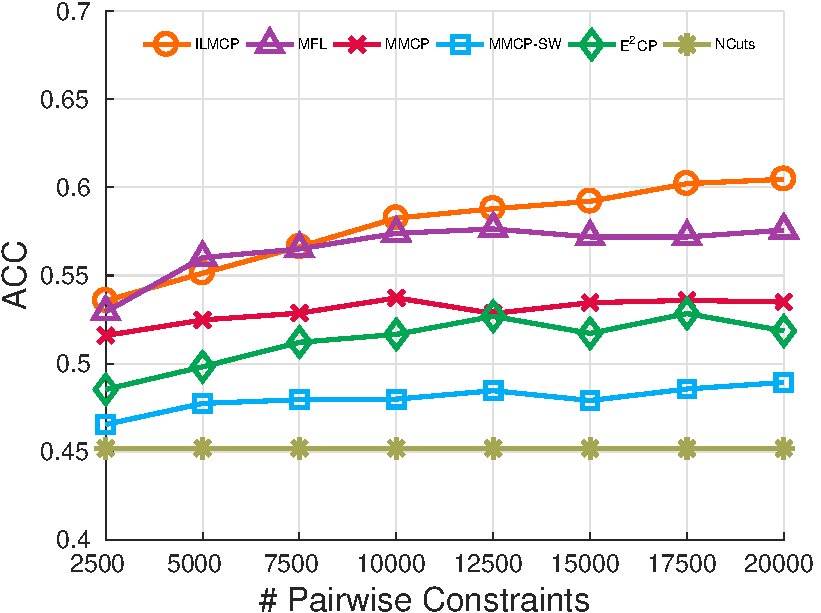
\includegraphics[width=0.49\textwidth]{chap4/corel5k_cn_acc_3.pdf}}
                    \label{fig4:3viewacc1}
	\bisubcaptionbox{Corel 5k数据集上的NMI结果}%
					{NMI on  Corel 5k}
                    [0.49\textwidth]{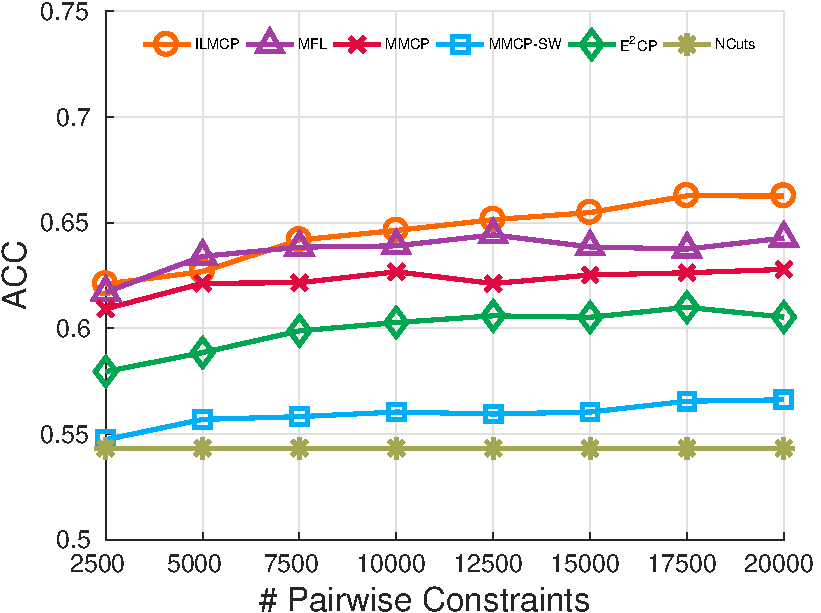
\includegraphics[width=0.49\textwidth]{chap4/corel5k_cn_nmi_3.pdf}}
                    \label{fig4:3viewnmi1}
                    
	\centering
	\bisubcaptionbox{PASCAL VOC'07数据集上的ACC结果}%
					{ACC on  PASCAL VOC'07}
					[0.49\textwidth]{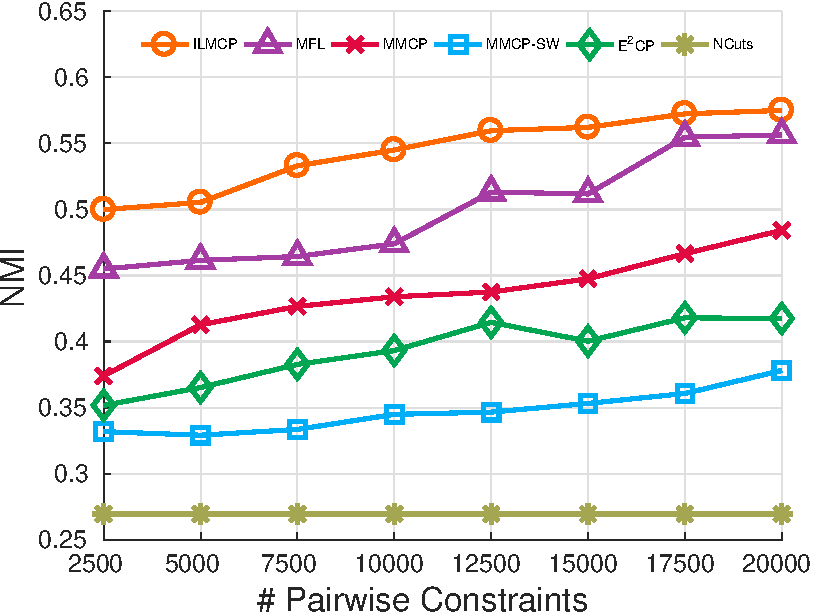
\includegraphics[width=0.49\textwidth]{chap4/voc_cn_acc_3.pdf}}
                    \label{fig4:3viewacc2}
	\bisubcaptionbox{PASCAL VOC'07数据集上的NMI结果}%
					{NMI on  PASCAL VOC'07}
					[0.49\textwidth]{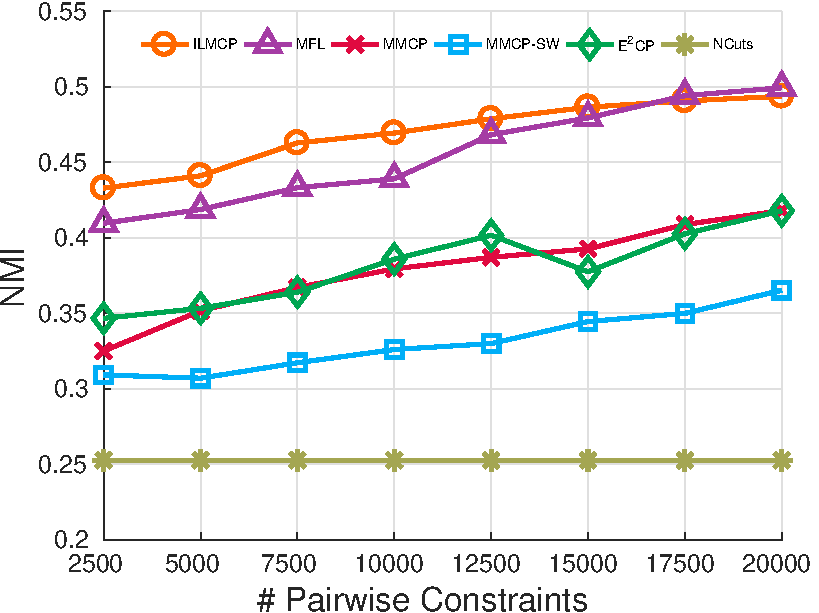
\includegraphics[width=0.49\textwidth]{chap4/voc_cn_nmi_3.pdf}}
                    \label{fig4:3viewnmi2}
	\bicaption{在Corel 5k和PASCAL VOC'07数据集上,不同约束数量下采用3个模态的聚类的ACC和NMI结果,需注意Y轴的尺度不相同}{Clustering result ACC and NMI on 3-modalities of Corel 5k and PASCAL VOC'07 with different numbers of pairwise constraints. Note the different Y-axis scales}
	\label{fig4:3view}
\end{figure} 


\begin{figure}[t]
	\centering
	\bisubcaptionbox{Corel 5k数据集上的ACC结果}%
					{ACC on  Corel 5k}
					[0.49\textwidth]{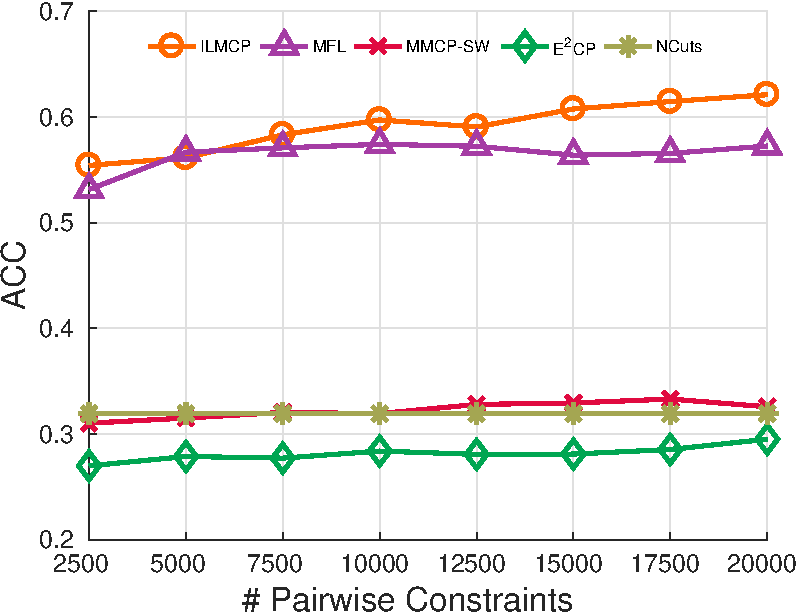
\includegraphics[width=0.49\textwidth]{chap4/corel5k_cn_acc_16.pdf}}
                    \label{fig4:16viewacc1}
	\bisubcaptionbox{Corel 5k数据集上的NMI结果}%
					{NMI on  Corel 5k}
                    [0.49\textwidth]{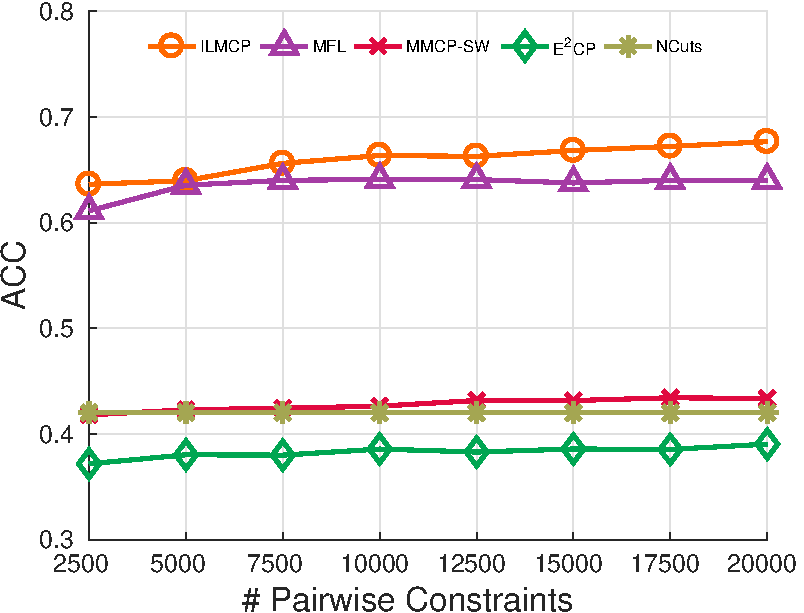
\includegraphics[width=0.49\textwidth]{chap4/corel5k_cn_nmi_16.pdf}}
                    \label{fig4:16viewnmi1}
                    
	\centering
	\bisubcaptionbox{PASCAL VOC'07数据集上的ACC结果}%
					{ACC on  PASCAL VOC'07}
					[0.49\textwidth]{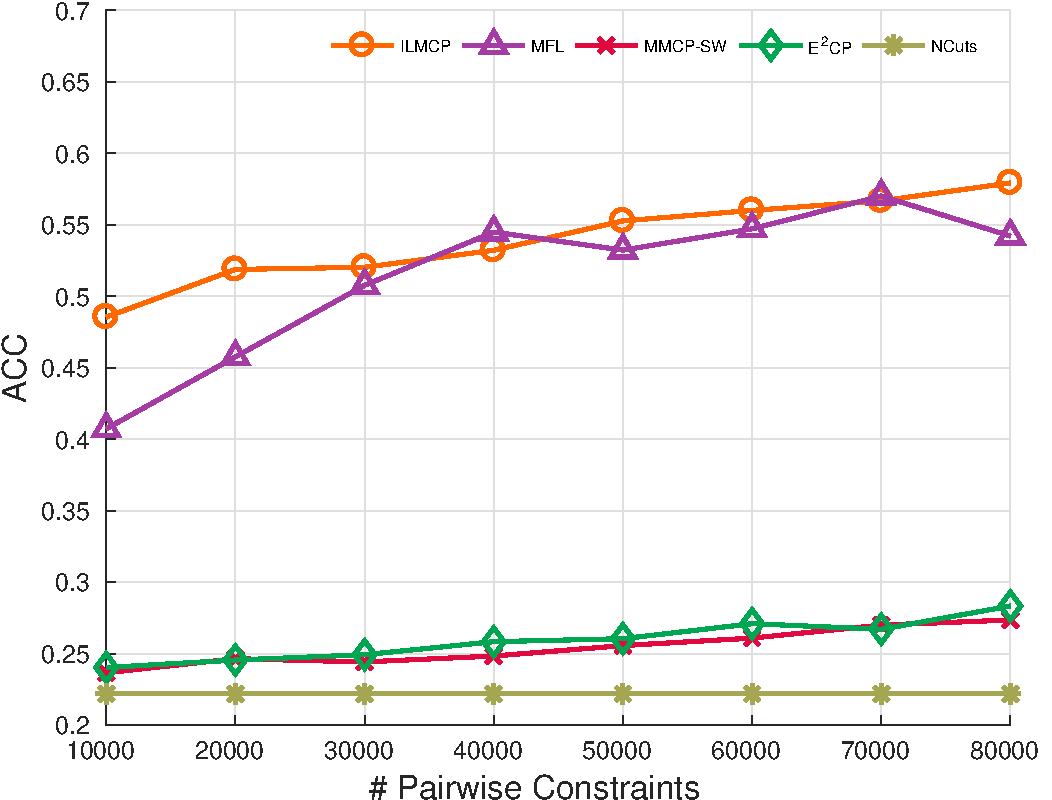
\includegraphics[width=0.49\textwidth]{chap4/voc_cn_acc_16.pdf}}
                    \label{fig4:16viewacc2}
	\bisubcaptionbox{PASCAL VOC'07数据集上的NMI结果}%
					{NMI on  PASCAL VOC'07}
					[0.49\textwidth]{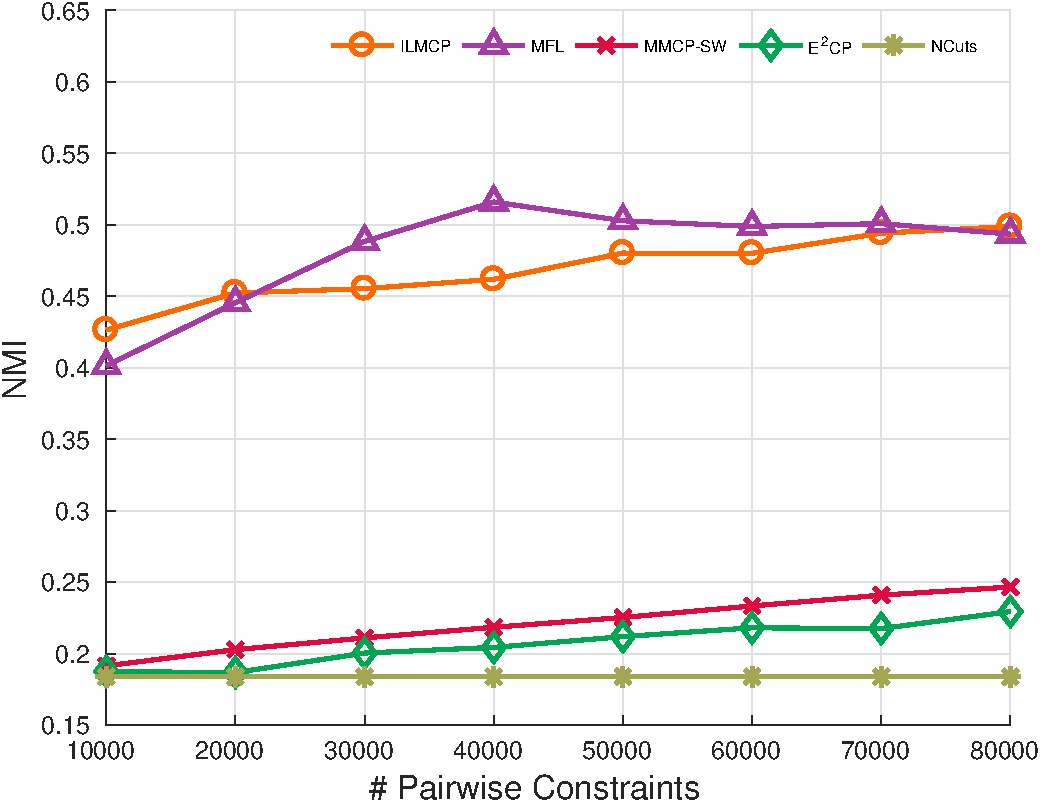
\includegraphics[width=0.49\textwidth]{chap4/voc_cn_nmi_16.pdf}}
                    \label{fig4:16viewnmi2}
	\bicaption{在Corel 5k和PASCAL VOC'07数据集上,不同约束数量下采用16个模态的聚类的ACC和NMI结果,需注意Y轴的尺度不相同}{Clustering result ACC and NMI on 16-modalities of Corel 5k and PASCAL VOC'07 with different numbers of pairwise constraints. Note the different Y-axis scales}
	\label{fig4:16view}
\end{figure} 

在本节的实验中,由于没有验证集可供在聚类实验中进行参数搜索,我们采用与MFL相同的固定参数选择标准。$k$-NN近邻数量被设为$ k = \mathrm{Round}(\mathrm{log}_2(\frac{n}{c}))$,其中$ n $为数据点数量,$ c $为聚类的数量。实验中采用传播参数$\eta = 0.25$。
我们对谱聚类的特征投影结果进行$k$-means聚类,将30次$k$-means聚类作为一轮,并选择类内和最小的聚类作为结果。在评估中,我们对每个算法随机生成了5个约束矩阵,对每个约束矩阵的约束传播的结果进行了5轮聚类,并在实验结果中报告了平均的聚类评估结果。



\begin{table}[t]
    \bicaption{在Corel 5k数据集上采用3个、8个和16个模态情况下20,000个成对约束的聚类性能}{Clustering performance of 3, 8 and 16 modalities on Corel 5k with 20,000 constraints}
    \label{tab4:modal}
    \centering
    \setlength{\tabcolsep}{8pt}
    \begin{tabular}{l*{6}{c}}
        \toprule
        &\multicolumn{2}{c}{3 modalities} & \multicolumn{2}{c}{8 modalities} & \multicolumn{2}{c}{16 modalities}\\
        \cmidrule(lr){2-3}
        \cmidrule(lr){4-5}
        \cmidrule(lr){6-7}
        & ACC\% & NMI\% & ACC\% & NMI\% & ACC\% & NMI\% \\
        \midrule
        NCuts\cite{shi2000normalized} & 44.98 & 54.33 & 38.61 & 49.27 & 32.07 & 42.11 \\ 
        E$^2$CP\cite{lu2010constrained} & 52.64 & 61.14 & 40.19 & 50.17 & 28.80 & 39.17 \\ 
        MCMCP\cite{fu2012modalities} & 49.15 & 59.90 & 36.72 & 51.56 & 36.24 & 51.12 \\ 
        MMCP\cite{fu2011multi} & 53.49 & 62.79 & - & - & - & - \\ 
        MMCP-SW\cite{fu2011multi} & 48.50 & 56.58 & 37.82 & 48.33 & 32.98 & 43.63 \\ 
        MFL & {56.36} & {63.99} & {57.04} & {64.11} & {56.67} &{ 64.09}\\
        ILMCP & \textbf{60.47} & \textbf{66.26} & \textbf{60.06} & \textbf{66.45 } & \textbf{62.12} &\textbf{ 67.67} \\
        \bottomrule
    \end{tabular}
\end{table}


\begin{table}[t]
    \bicaption{在PASCAL VOC'07数据集上采用3个、8个和16个模态情况下80,000个成对约束的聚类性能}{Clustering performance of 3, 8 and 16 modalities on PASCAL VOC'07  with 80,000 constraints}
    \label{tab4:modal2}
    \centering
    \setlength{\tabcolsep}{8pt}
    \begin{tabular}{l*{6}{c}}
        \toprule
        &\multicolumn{2}{c}{3 modalities} & \multicolumn{2}{c}{8 modalities} & \multicolumn{2}{c}{16 modalities}\\
        \cmidrule(lr){2-3}
        \cmidrule(lr){4-5}
        \cmidrule(lr){6-7}
        & ACC\% & NMI\% & ACC\% & NMI\% & ACC\% & NMI\%  \\
        \midrule
        NCuts\cite{shi2000normalized}  & 26.76 & 25.04 & 23.07 & 21.26 & 22.31 & 18.40  \\ 
        E$^2$CP\cite{lu2010constrained}  & 40.46 & 39.50 & 29.39 & 26.40 & 25.66 & 21.29 \\ 
        MCMCP\cite{fu2012modalities} & 34.85 & 27.34 & 29.36 & 24.79 & 29.80 & 24.98  \\ 
        MMCP\cite{fu2011multi}  & 48.42 & 41.80 & - & - & - & - \\ 
        MMCP-SW\cite{fu2011multi} & 38.29 & 36.14 & 29.04 & 26.40 & 27.85 & 24.90 \\ 
        MFL  & {56.66} & \textbf{49.98} & {54.95} & {49.06} & {56.35} &{49.86}\\
        ILMCP & \textbf{57.51} & {49.38} & \textbf{57.63} & \textbf{49.49} & \textbf{57.93} & \textbf{49.88} \\
        \bottomrule
    \end{tabular}
\end{table}

\subsection{性能评估与比较}
在本节中,我们进行了五个实验以实现对所提出算法的聚类性能评估。

为与专为2种模态情况设计的算法进行比较,我们在2种模态的情况下测试了ILMCP方法,并在表\ref{tab4:2case}中对比了不同算法的性能。由于MSCP和UCP方法使用约束传播结果来对每个模态的相似性矩阵进行分别调整,因此没有像ILMCP中${W^*}$矩阵这样的统一的相似性矩阵作为最终结果。我们对这两种算法分别在每个模态的相似性上聚类并给出了评估结果,这两种算法都在传播调整过的文本描述特征上取得了各自的最优表现。可以注意到,在所有对照方法中所提出的ILMCP具有最佳的聚类性能。
由于从是文本描述中提取的特征,模态\textit{tags}在聚类中显示出压倒性的优势。基于这点观察结果,我们针对不使用文本描述信息的2种模态情况进行了更多的实验。表\ref{tab4:2modal_notag}报告了不使用\textit{tags}特征,而采用\textit{DenseSift} 和 \textit{Gist}作为2种模态信息的情况下的聚类性能对照结果。

\begin{table}[t]
    %		\small
    \centering
    \bicaption{E$^2$CP和ILMCP方法在Corel 5k 和 PASCAL VOC'07数据集上的聚类性能表现(ACC和NMI)}{Clustering performance (ACC and NMI) on of E$^2$CP and ILMCP on Corel 5k and PASCAL VOC'07.}
    %\begin{sc}
    \setlength{\tabcolsep}{15pt}
    \begin{tabular}{lcccccc}
        \toprule
        &\multicolumn{2}{c}{Corel 5k} & \multicolumn{2}{c}{Pascal Voc'07} \\
        \cmidrule(lr){2-3}
        \cmidrule(lr){4-5}
        & ACC\% & NMI\% & ACC\% & NMI\% \\
        \midrule
        E$^2$CP\cite{lu2010constrained}: &&&&\\
        DenseSift & 24.40 & 36.44 & 25.34 & 22.80 \\ 
        Lab & 18.39 & 27.10 & 16.56 & 9.11 \\ 
        tags & 51.44 & 60.30 & 51.92 & 44.98 \\ 
        Hsv & 25.83 & 35.61 & 16.86 & 8.42 \\ 
        Gist & 12.99 & 22.04 & 22.32 & 16.22 \\ 
        RgbV3H1 & 20.79 & 31.03 & 18.37 & 11.14 \\ 
        HarrisSiftV3H1 & 9.00 & 13.75 & 23.53 & 17.43 \\ 
        HsvV3H1 & 25.54 & 35.01 & 17.22 & 9.06 \\ 
        HarrisSift & 12.01 & 18.09 & 24.68 & 19.04 \\ 
        DenseHueV3H1 & 18.38 & 27.92 & 16.09 & 8.68 \\ 
        DenseSiftV3H1 & 18.33 & 27.64 & 28.51 & 27.10 \\ 
        DenseHue & 17.24 & 27.54 & 16.63 & 8.84 \\ 
        LabV3H1 & 22.97 & 36.55 & 18.02 & 9.58 \\ 
        HarrisHue & 15.72 & 26.17 & 16.38 & 9.04 \\ 
        HarrisHueV3H1 & 15.58 & 25.93 & 17.05 & 9.05 \\ 
        Rgb & 19.69 & 30.33 & 16.77 & 9.12 \\ 
        \midrule
        ILMCP: &&&&\\
        3-modalities         & {60.47} & {66.26}  & {57.51} & {49.38} \\ 
        16-modalities         &\textbf{62.12} &\textbf{ 67.67}   & \textbf{57.93} & \textbf{49.88}   \\	
        \bottomrule
    \end{tabular}
    \label{tab4:e2cp}
\end{table}

3种模态和16种模态情况下不同约束数量对应的聚类结果如图\ref{fig4:3view}及图\ref{fig4:16view}中所示。
所采样出的用于传播的约束数量是Corel 5k和PASCAL VOC'07数据集中所有约束总数的$0.01\%$至$0.08\%$,间隔为$0.01\%$。我们在3种模态的实验中同样考虑了两种不同版本的MMCP方法。一种是原始的MMCP,其中我们依据文献\parencite{fu2011multi}中提出的3种模态的先验概率,将其设置为0.2、0.05和0.75。由于在实际情况中很难确定每个模态的重要性,所以另一个版本是采用相同权重的MMCP(MMCP-SW),在其中每个模态被分配了相同的先验概率。
在对E$^2$CP的实验中我们分别对每一个模态独立地进行约束传播,然后通过线性组合将传播后的相似性矩阵进行融合。通过图\ref{fig4:3view}可以看到,在同时利用3种模态的情况下,所提出的ILMCP聚类性能明显超过其他对照算法。在图\ref{fig4:16view}中虽然少部分情况下MFL方法效果略优,但ILMCP的整体稳定性和聚类性能都有明显优势。

表\ref{tab4:modal}和表\ref{tab4:modal2}显示了不同模态数量情况下的更详细的聚类评估结果。当具有8种或16种模态时,通过手工方式确定每种模态的重要性变得几乎无法实现。 因此,在MMCP中我们令每个模态都具有相同的先验图概率$1/8$和$1/16$,即MMCP-SW。从定量结果可以看出,随着模态数量的增加,聚类的任务由于没有监督信息反而变得更加困难。同时ILMCP的优势也更加明显。

我们将所提出的方法与每种模态独立进行约束传播的结果进行比较。如表\ref{tab4:e2cp}所示,我们对具有$0.08\%$的成对约束的16种模态的相似性分别采用E$^2$CP算法进行约束传播。同时表\ref{tab4:e2cp}也给出了3种模态情况和16种模态情况下的ILMCP聚类结果,以供对照参考,这些结果与图\ref{fig4:3view}、图\ref{fig4:16view}、表\ref{tab4:modal}和表\ref{tab4:modal2}中所展示的数据结果相同。
可以看出,在两个数据集中,采用文本描述特征作为唯一模态均具有最佳性能。但是,在实际应用中由于不存在监督数据,因此并不能明确哪个模态下的特征信息能取得更令人满意的结果。

表\ref{tab4:path}展示了所提出方法不同部分对应的消融实验的实验结果。可以发现,所提出的相容条件概率分布重构(CCDR),即不同模态边缘概率的学习部分,提供了$21.79\%$的NMI提升,和$23.35\%$的ACC提升,起到了最主要作用。
ILMCP所包含的相容条件概率分布重构(CCDR)、约束数据均衡(Balance)和整流Sigmoid函数(Re-Sig)三个部分均对最终结果有提升效果。
\begin{table}[t]
    %		\small
    \centering
    \bicaption{从MMCP方法到ILMCP方法的消融实验(Corel 5k数据集中的16个模态)}{The path from MMCP to ILMCP (on Corel 5k with 16-modalities)}
    %	\footnotesize
    \label{tab4:path}
    %\begin{sc}
    %	\begin{tabular}{c| p{30pt}<{\centering}  p{30pt}<{\centering}  p{30pt}<{\centering} |p{20pt}<{\centering}  p{20pt}<{\centering} }
    
    \setlength{\tabcolsep}{8pt}
    \begin{tabular}{lccccc}
        \toprule
        
        & CCDR? & { Balance?}& {Re-Sig?}& ACC\%&NMI\% \\		 
        \midrule
        MMCP-SW\cite{fu2011multi}&&&&32.98 & 43.63\\
        \midrule
        &&& & 33.32 & 43.14 \\ 
        &&&\checkmark & 35.19 & 43.28 \\ 
        &&\checkmark& & 34.01 & 44.01 \\ 
        interim methods&&\checkmark&\checkmark& 35.76 & 43.79 \\ 
        &\checkmark&&& 56.67 & 64.93 \\ 
        &\checkmark&&\checkmark& 59.44 & 66.06 \\ 
        &\checkmark&\checkmark&& 57.18 & 65.96 \\ 
        \midrule
        ILMCP&\checkmark&\checkmark&\checkmark& \textbf{62.12} & \textbf{67.67} \\ 
        \bottomrule
    \end{tabular}
    %\end{sc}
\end{table}

\subsection{模态选择}
由于所提出的方法可以用于衡量每个模态的重要性,我们可以将ILMCP视为模态选择的一个可行的引导信息。在该方法中,可以直接生成每个图的边缘概率$ P(\mathcal{G}_s)$。通过对每个模态对应的图的边缘概率进行排序,即可以剔除具有最小概率的模态。按照上述策略,我们可以对所有模态进行一一消除,并测试每一步后的聚类效果。图\ref{fig4:corel5k_1_10}显示了进行了模态选择后的聚类性能,其中我们根据图的边缘概率从小到大的顺序逐渐删除了16个模态中的15个。当我们开始根据其低边缘概率去除一些噪声较多的模态时,在数据集PASCAL VOC'07上的聚类性能会略有提高,但基本保持稳定,这是由于所提出的算法策略可会赋予噪声高的模态更低的概率,以免受噪声影响整体效果。当我们继续消除更多的模态时,某些包含判别性信息较多的模态将被删除,性能将会开始下降,逐渐失去多模态学习的优势。 图\ref{fig4:corel5k_1_10}中的结果说明了所提出的方法在大多数情况下均能达到预期的结果。

\begin{figure}[t]
    \centering
    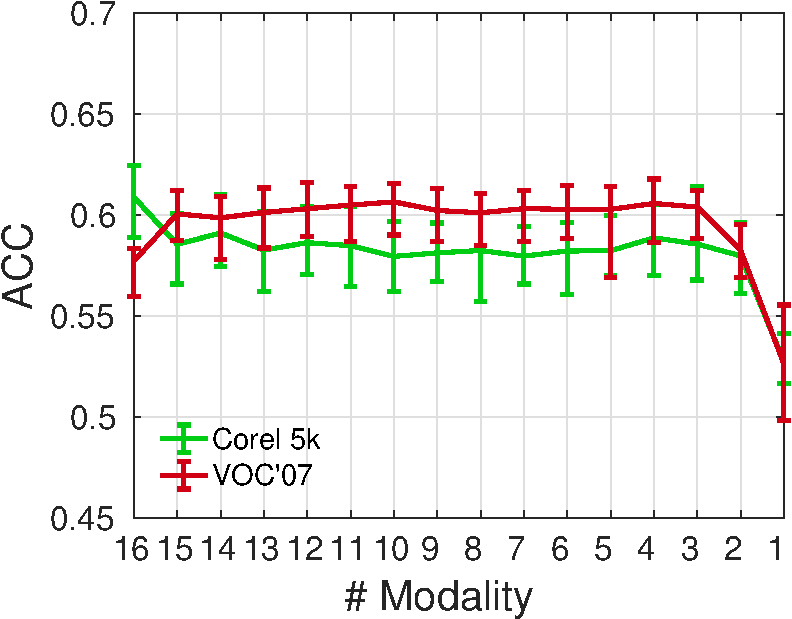
\includegraphics[width=0.49\textwidth]{chap4/corel5k_voc_1_16_acc.pdf}
    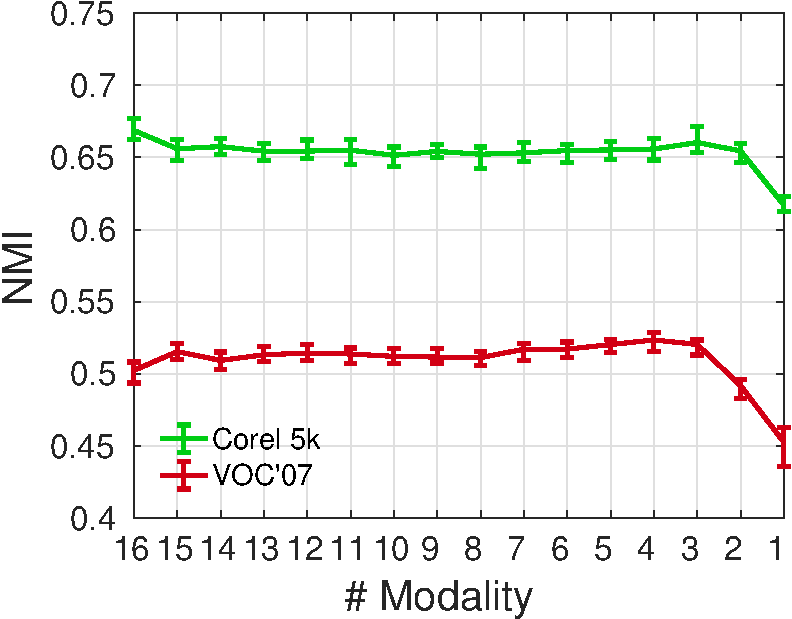
\includegraphics[width=0.49\textwidth]{chap4/corel5k_voc_1_16_nmi.pdf}
	\bicaption{Corel 5k 和 PASCAL VOC'07数据集上的模态选择结果}{Modality selection results on Corel 5k and PASCAL VOC'07}
	\label{fig4:corel5k_1_10}
\end{figure} 

\section{本章小结}
在本章中,我们提出了一种新颖的多模态约束传播方法,称为实例级多模态约束传播(ILMCP)。在所提出的方法通过从实例级的相容条件概率分布中学习多模态数据集下的统一的数据相似性,并且缓解了约束传播中的成对约束数据量不均衡的问题。
大量实验证明了该方法的优越性。由于多模态融合在结构学习中是一个流行的趋势。利用基本的CCDR问题来进行基于深度神经网络的多模态相似性传播,并将传播结果用于结构嵌入学习是未来值得研究的工作之一。